\section{Examples}\label{sec:examples}


\subsection{Hello \textit{entangled} world!}

Consider a simple quantum program that creates the so-called Bell state:

\begin{minted}[fontsize=\footnotesize]{ruby}
allocate q1:
  mix q1
  allocate q2:
    entangle q1 q2
  measure collect
measure collect
\end{minted}

This program illustrates qstack's core syntax elements:

\textbf{Quantum instructions (gates):} Instructions like \texttt{mix} and \texttt{entangle} are quantum operations that manipulate quantum states. These belong to qstack's ``toy instruction set''—a collection of intuitively named gates designed for accessibility. The \texttt{mix} operation creates a superposition state where a qubit exists as both $0$ and $1$ simultaneously until measured. The \texttt{entangle} operation creates quantum correlation between qubits—when entangled, measuring one qubit instantly determines the state of the other, producing perfectly correlated outcomes. (We explore how these operations map to standard quantum gates in Section~\ref{sec:synthesis}.)

\textbf{Nested kernels:} A kernel can appear anywhere an instruction is expected, enabling dynamic program structure. In our example, the inner kernel \texttt{allocate q2: entangle q1 q2; measure collect} is itself an instruction within the outer kernel. This nesting allows qubits to be allocated precisely when needed and measured when their quantum properties are no longer required.

\textbf{Measurement and callbacks:} When a kernel completes its instructions, it measures its allocated qubit, which has several effects: the qubit is deallocated from the quantum system, any entanglement with other qubits causes those qubits to potentially collapse into a subset of their possible states, and the classical measurement result ($0$ or $1$) is passed to the specified callback function. In our Bell state example, both measurements use the \texttt{collect} callback, which simply stores each result on a classical stack without generating additional quantum computation.

When this Bell state program runs in a noiseless environment, the expected outcome is perfectly correlated measurement results: both qubits will measure as $0$ about $50\%$ of the time, and both will measure as $1$ about $50\%$ of the time. Unless there is noise, you will never see mixed results like $(0,1)$ or $(1,0)$ because the qubits are entangled. This correlation demonstrates that quantum entanglement creates dependencies between measurement outcomes that don't exist in classical systems.


\begin{figure}[h]
\centering
\begin{subfigure}{.49\textwidth}
  \centering
  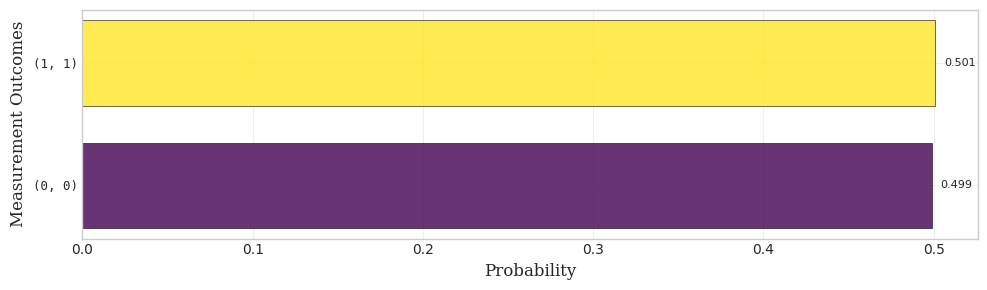
\includegraphics[width=\linewidth]{figures/bell_state_histogram.png}
  \caption{Bell state measurement outcomes}
  \label{fig:bell-state-sub}
\end{subfigure}%
\begin{subfigure}{.49\textwidth}
  \centering
  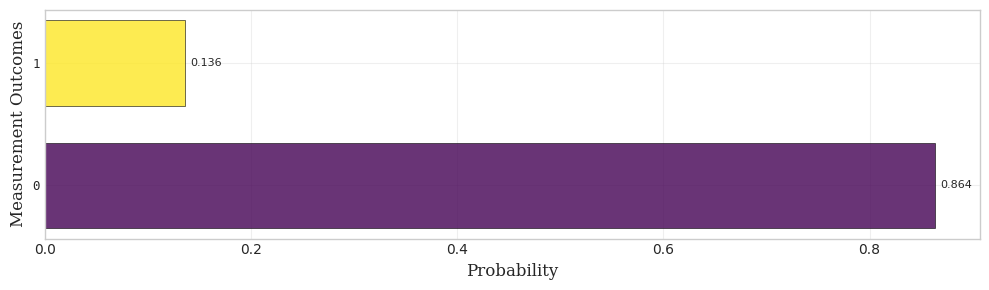
\includegraphics[width=\linewidth]{figures/t_gate_histogram.png}
  \caption{T-gate measurement outcomes}
  \label{fig:t-gate-sub}
\end{subfigure}
\caption{Measurement outcomes from simulation of two key quantum programs: (a) The Bell state program shows the perfectly correlated outcomes where both qubits measure as $0$ (represented as `(0,0)') or as $1$ (represented as `(1,1)') with 50\% probability each. The absence of mixed outcomes (`(0,1)' or `(1,0)') demonstrates quantum entanglement. (b) The T-gate implementation shows the distinctive probability distribution that results from applying a T-gate to a qubit in superposition, with approximately $\cos^2(\pi/8) \approx 85\%$ probability for outcome `0' and $\sin^2(\pi/8) \approx 15\%$ probability for outcome `1'.}
\label{fig:quantum-histograms}
\end{figure}


\subsection{Creating Magic}

This example demonstrates qstack's ability to perform advanced quantum operations through classical feedback. We implement a T-gate—a crucial operation for universal quantum computation that cannot be efficiently simulated classically.

The T-gate applies a phase rotation ($\pi/4$) that takes a qubit outside the ``Clifford group'' of operations. Operations beyond this group make the computation truly quantum and classically hard to simulate. While essential for universal quantum computing, T-gates are challenging to implement directly on many quantum hardware platforms and are typically synthesized through combinations of more accessible operations.

One approach to implementing the T-gate uses a technique called ``state injection'' with special resource states known as ``magic states.'' The process involves:

\begin{itemize}
\item Prepare a special resource state (the ``magic T-state'')
\item Entangle it with our target qubit
\item Measure the resource qubit
\item Apply a conditional correction based on the measurement result
\end{itemize}

Here's how this looks in qstack:

\begin{minted}[fontsize=\footnotesize]{ruby}
allocate target:
  mix target          
  allocate resource:
    prepare_t_state resource      
    entangle target resource      
  measure t_correction(target_qubit=target)    
  mix target
measure collect                   
\end{minted}

The \texttt{t\_correction} callback is defined as:

\begin{minted}[fontsize=\scriptsize]{python}
def t_correction(measurement, target_qubit):
    if measurement == 1:
        # Apply correction operation (S gate) only if we measured 1
        return Kernel(
          allocate:
            s target_qubit
          measure
        )
    else:
        # No correction needed if we measured 0
        return None
\end{minted}


This program demonstrates a fundamental concept in fault-tolerant quantum computation: we can implement hard-to-synthesize gates (like T) by preparing special resource states, performing entanglement and measurement, and then applying classical feedback to correct the final state. The measurement of the resource qubit is random, showing $0$ or $1$ with equal probability (50\% each). However, the measurement of the target qubit after the entire procedure exhibits the distinctive probability distribution of a T-gate applied to a qubit in superposition: approximately $\cos^2(\pi/8) \approx 85\%$ probability of measuring $0$ and $\sin^2(\pi/8) \approx 15\%$ probability of measuring $1$. The callback applies a conditional correction (S-gate) only when the first measurement outcome is $1$, which is necessary to ensure the target qubit properly receives the phase information from the resource state.

In practice, these T-states are themselves difficult to prepare perfectly and often require additional purification procedures. The ability to express this pattern of state preparation, measurement, and conditional correction demonstrates how qstack's callback mechanism naturally accommodates advanced quantum computing techniques.


\subsection{Majority vote}\label{sec:majority-vote}

Critical for quantum error correction is the ability to compile quantum programs into versions that encode a single qubit using multiple physical qubits, and that insert arbitrary classical computation into the program, without affecting its semantics.

It is important to note that the simple repetition code presented here is \textit{not} a valid quantum error correction technique in practice, as it only addresses bit-flip errors but not phase-flip errors that also occur in real quantum systems. We use it purely for pedagogical purposes to illustrate qstack's program transformation capabilities. Proper quantum error correction codes (like the Steane code, which we discuss in section~\ref{sec:error-correction}) follow similar principles but with more sophisticated encoding and decoding procedures.

Consider this simple program that returns $1$ by applying a \texttt{flip} operation to a qubit:

\begin{minted}[fontsize=\footnotesize]{ruby}
allocate q:
  flip q
measure
\end{minted}

In an ideal quantum computer, this program always returns $1$. However, in real quantum hardware, operations are subject to noise. If the error rate for a flip operation is $p$, the program returns $0$ (incorrect) with probability $p$ and $1$ (correct) with probability $1-p$.

To increase reliability, we can implement a simple repetition code that encodes a single logical qubit using three physical qubits. By applying the \texttt{flip} operation to each qubit and determining the final outcome through majority voting, we reduce the error probability from $p$ to approximately $3p^2(1-p) + p^3$ when $p < 0.5$. With $p = 0.1$, the error rate drops from 10\% to approximately 2.8\%.

Our redundancy-enhanced program can be compiled as:

\begin{minted}[fontsize=\footnotesize]{ruby}
allocate q.1 q.2 q.3:
    flip q.1
    flip q.2
    flip q.3
measure vote
\end{minted}

with the \texttt{vote} callback defined as:

\begin{minted}[fontsize=\scriptsize]{python}
def vote(context):
    m1, m2, m3 = context.pop(3)
    
    if (m1 + m2 + m3) >= 2:
        context.push(1)  # Majority voted for 1
    else:
        context.push(0)  # Majority voted for 0
    
    return None
\end{minted}

The new program uses three physical qubits instead of one to gain redundancy. The \texttt{vote} callback performs a critical transformation: it consumes the three individual measurement outcomes from the stack using \texttt{context.pop()}, computes their majority vote, and places a single logical result back onto the stack with \texttt{context.push()}. This process illustrates what measurement accomplishes in qstack: when a qubit is measured, it is deallocated from the quantum system, any entanglement with remaining qubits causes those qubits to potentially collapse into a subset of their possible states, and the classical measurement result ($0$ or $1$) is passed to the callback function for processing.

The \texttt{vote} callback's replacement of three physical measurements with one logical measurement is the essence of error correction. Since \texttt{vote} returns \texttt{None} rather than a new kernel, no additional quantum instructions are executed after the measurement—the error correction happens entirely in the classical processing. As such, the program's observable behavior remains identical to the original: a single measurement outcome on the stack, preserving the program's semantics despite the added complexity.

The measurement stack plays a central role in qstack programs. Quantum measurements populate the stack with classical bits, and classical callbacks can manipulate it by consuming, transforming, or replacing these measurements. In error correction scenarios like the one above, measurements from multiple physical qubits are processed by a callback that pushes only a single logical measurement outcome onto the stack—effectively hiding the complexity of error correction from the rest of the program.

In the previous example, we can also see some of the syntactic sugar available in qstack. Notice how multiple qubits can be allocated in a single statement (\texttt{allocate q.1 q.2 q.3:}) rather than requiring nested kernels for each qubit. It's worth noting that \texttt{collect} is the default callback for intermediate measurements when none is explicitly specified. This means that the measurement results are simply stored on the stack without triggering additional quantum operations. For instance, the Bell state example could have been written as:

\begin{minted}[fontsize=\footnotesize]{ruby}
allocate q1 q2:
  mix q1
  entangle q1 q2
measure
\end{minted}

On the other hand, when working with multi-qubit measurements, callbacks like \texttt{vote} automatically read their arguments from the measurement stack. When multiple qubits are measured together, their measurement results are pushed onto the stack in the order they were measured (last measured qubit's result is on top), and the callback then consumes these values from the stack. This behavior is evident in the \texttt{vote} callback implementation, which uses \texttt{context.pop(3)} to retrieve all three measurement results at once, processes them, and then pushes a single result back onto the stack with \texttt{context.push()}.

While we've shown the error-corrected version of our simple flip program directly, it's important to understand that in qstack, such transformations aren't written by hand. Instead, qstack exposes this encoding as a compiler pass that can be applied to any quantum program. This approach separates the concerns of algorithm design from error correction implementation. The programmer writes a clean, logical algorithm without redundancy, and the compiler automatically transforms it into an error-corrected version. This transformation handles both the quantum operations (expanding qubits and gates, for example) and the classical processing (injecting appropriate callback decoding functions), enabling a modular approach to quantum programs compilation where error correction can be applied or modified without changing the core algorithm.

\subsection{Compositional Compilation}

As such, a key advantage of qstack's design is the compositionality of its compiler framework. Building on the previous explanation, let's explore in more detail how these transformations work in practice. To demonstrate this, we'll transform our T-gate implementation from earlier through multiple compilation stages to add error correction.

Let's see how this works with our T-gate program:

\begin{minted}[fontsize=\scriptsize]{python}
from qstack import Program
from qstack.compilers.toy2cliffords import ToyCompiler
from qstack.compilers.rep3_trivial import TrivialRepetitionCompiler

from examples.t_gate import t_gate_program, t_gate_callbacks

# First transform toy gates to canonical gates
canonical_compiler = ToyCompiler()
canonical_program, canonical_callbacks = canonical_compiler.compile(t_gate_program, t_gate_callbacks)

# Then apply 3-qubit repetition code
rep3_compiler = TrivialRepetitionCompiler()
error_corrected_program, error_corrected_callbacks = rep3_compiler.compile(canonical_program, canonical_callbacks)
\end{minted}

This example demonstrates a two-stage compilation process. First, the ToyCompiler transforms the intuitive toy instruction set (with operations like \`{mix} and \`{prepare\_t\_state}) into the canonical instruction set of standard quantum gates (like Hadamard and CNOT). Since the TrivialRepetitionCompiler works only with canonical gates, this first transformation is necessary before the encoding can be applied. We discuss the specifics of gate synthesis and decomposition in Section~\ref{sec:synthesis}, so we'll focus here on the second transformation.

The repetition code compiler transforms the program in several critical ways:

\begin{itemize}
\item Each logical qubit (\texttt{target} and \texttt{resource}) is expanded into three physical qubits (e.g., \texttt{target.0}, \texttt{target.1}, \texttt{target.2})
\item Each quantum gate operation is replicated across the corresponding physical qubits
\item Measurements are transformed to use error correction via the \texttt{decode} callback
\item Most importantly, the \texttt{t\_correction} callback is automatically adapted to work with the error-corrected qubits
\end{itemize}

The transformation of callbacks demonstrates qstack's capability for abstraction. The compiler wraps the original callback in a new version that understands the expanded qubit naming scheme and applies the appropriate error correction. When \texttt{t\_correction} returns a kernel containing an S-gate operation on the original \texttt{target} qubit, the compiler automatically compiles this kernel just-in-time to apply the S-gate to all three physical qubits representing the logical \texttt{target}.

As noted in the majority vote example, the TrivialRepetitionCompiler does not implement true quantum error correction—it is a simplified encoding that would not protect against phase errors in a real quantum system. In a real application, this trivial compiler could be replaced with a quantum error correction compiler implementing codes like the Surface code or Steane code, without changing the program's structure.



The callback transformation creates this compilation pattern:

\begin{minted}[fontsize=\scriptsize]{python}
# Original callback chain (simplified representation)
t_correction(target_qubit=target) -> collect

# After repetition code transformation
decode | _rep3-trivial_:t_correction(target_qubit=target) -> _rep3-trivial_:collect
\end{minted}

The \texttt{decode} callback performs majority voting on the three physical measurements to determine the logical measurement result, then passes this to the transformed original callback. Any new kernel returned by the callback is automatically compiled by the \texttt{\_rep3-trivial\_} transformation to work with the three-qubit encoding.

This approach demonstrates qstack's compositionality—program transformation occurs at compile time, and both quantum operations and classical control are automatically adapted. Programmers can write quantum algorithms without addressing error correction details, applying it as a separate compilation step.

% Moreover, the new program can be encoded again using the same schema, generating a 9-qubit program:

% \begin{minted}{ruby}
% allocate q.1.1 q.1.2 q.1.3:
%     allocate q.2.1 q.2.2 q.2.3:
%         allocate q.3.1 q.3.2 q.3.3:
%             flip q.1.1
%             flip q.1.2
%             flip q.1.3
%             flip q.2.1
%             flip q.2.2
%             flip q.2.3
%             flip q.3.1
%             flip q.3.2
%             flip q.3.3
%         measure vote
%     measure vote
% measure vote 
% ---
% vote
% \end{minted}

% This creates a concatenated error correction scheme where each logical qubit from the first level is itself encoded using three physical qubits. The nested \`{vote} callbacks cascade the error correction: the innermost callback processes the 9 physical measurements into 3 logical measurements, the middle callback further condenses these into a single logical measurement, and the outermost callback processes this result. Despite the complexity of using 9 physical qubits and multiple layers of error correction, the program's semantics and observable behavior remain identical to the original single-qubit version, a testament to the composability of error correction in qstack's kernel-based model.

% The examples in this section have demonstrated qstack's fundamental programming patterns and error correction capabilities. In the next section, we will explore how qstack handles instruction synthesis and decomposition, which is essential for targeting different quantum hardware platforms.
